\chapter{Phage therapy and antibiotics for biofilm eradication: a predictive model}
%\abstract{
Bacteria that make up the complex physical structures known as biofilms can be 10-1000 fold more resistant to antibiotics than planktonic (free-living) bacteria.  In this chapter we develop a mathematical model to analyze therapeutic techniques that have been proposed to reduce and/or eradicate biofilms, specifically, antibiotics and phage therapy. In this context, the biofilm can be understood as a group defense mechanism, such that the functional response of phages to the biofilm bacterial density is reduced as the biofilm approaches carrying capacity. To capture this mechanism we introduce the function $f(x)=\left(\kappa-\frac{x}{K}\right)x,$ where $x$ is biofilm density, $K$ is biofilm carrying capacity and $1<\kappa <2$ is the group defense parameter. The model predicts that two therapeutic strategies of recent experimental interest (phage therapy followed by antibiotics, or antibiotics followed by phage therapy) can reduce but not eradicate the biofilm.  In contrast, we predict that complete elimination of biofilm bacteria can be achieved by mechanisms that block the attachment of planktonic bacteria to the biofilm.
%}
\section{Introduction}
Bacteria are ubiquitous unicellular organisms, with critical importance in both human health and disease \citep{abedon_bacteriophage_2008}. Bacteria can exist as planktonic (free-living) cells, or in complex communities known as biofilms.  In the biofilm state, the bacterial colony is attached to a surface; within the biofilm each cell is sessile and surrounded by extracellular polymeric substances (EPS), substances produced by bacteria in the colony that determine the physical and chemical properties of the biofilm \citep{harper_bacteriophages_2014}. Biofilms are responsible for a variety of problems in water distribution systems \citep{douterelo_dynamics_2016}, the food industry \citep{van_houdt_biofilm_2010}, and medical treatment \citep{omar_microbial_2017, ciofu_antibiotic_2017}.  Most importantly, biofilms have been implicated as a key factor in two-thirds of human infections \citep{fux_bacterial_2003}. \\

Bacteria are able to rapidly develop resistance against agents employed to eradicate them. %This resistance may be genotypic, phenotypic or a combination of both.  Genotypic resistance is inherited resistance through changes to the genetic code, while phenotypic resistance is due to a change in the phenotype (current physical characteristics) of the bacterial cell. One of the most important causes of phenotypic resistance is the physical structure of bacterial population \citep{sanchez-romero_contribution_2014}, called biofilm. 
In particular, bacteria in a biofilm have been shown to increase resistance to antibiotics by factors of ten to 1000 \citep{davies_understanding_2003}. Amongst the reasons for enhanced resistance in the biofilm state is the EPS structure surrounding the biofilm colony, which can completely block the infiltration of antibiotics, and the presence of persister cells in the biofilm colony, which are in a metabolically inactive state and thus protected from antibiotic action \citep{davies_understanding_2003}.\\

The goal of reducing or eradicating biofilm populations has been the focus of research over many years, and there has been much experimental work in this regard \citep{fleming_approaches_2017, ciofu_antibiotic_2017, feng_bacterial_2015}. Many agents have been employed for this purpose, which include but are not limited to natural inhibitors of biofilm, for example honey \citep{lee_low_2011}, %jakobsen_ajoene_2012}, 
drugs (antibiotics, biofilm-degrading components) \citep{lynch_new_2010, mu_potent_2016}, bacteriophages and phage-derived enzymes \citep{azeredo_use_2008, fernandez_low-level_2017, abedon_ecology_2015} or combinations of some of these \citep{chaudhry_synergy_2017}.  While phage therapy has been proposed as possibly the most effective of these agents, phages alone may not be sufficient to completely eradicate a biofilm\citep{abedon_ecology_2015}. Most recently, experimental work demonstrated that
%was carried out to investigate the question ``How does one deal with the increasing frequency of pathogens that are genetically resistant to multiple antibiotics and phenotypically resistant because of the physical  structure of their population?" \citep{chaudhry_synergy_2017}. They used some therapeutic strategies to overcome the resistance. They claimed 
using phage therapy first, followed by antibiotics, maximized the killing of bacteria in an established biofilm.\\

In this chapter, we develop a mathematical model to study these therapeutic strategies in detail.  In section 2.2, we develop the model, tracking biofilm and planktonic bacteria in two linked compartments. In section 2.3, we explore therapeutic strategies including: phage followed by antibiotics; antibiotics followed by phage; and a novel strategy we propose which may have the potential to eradicate the biofilm. In section 2.4, we derive some conclusions from our analysis.

\section{Mathematical model}

We model the interaction between bacteria and bacteriophages (viruses that infect bacteria) using an established predator-prey approach \citep{lenski_dynamics_1988}. %For this purpose we divide bacteria into biofilm and planktonic compartments.  
Our model considers cells of a single bacterial species in either a biofilm or planktonic compartment.   The model studies the population dynamics of biofilm cells, $B$, planktonic cells, $P$ and phage, $V_B$ and $V_P$, in the biofilm and planktonic compartments respectively.  The parameters of the model are described as follows.\\
 
The bacterial populations (biofilm or planktonic) are modeled as cell densities per unit volume, cells/cm$^3$. The biofilm population can increase logistically with a maximum growth rate $r$, but is limited by a fixed number of available attachment sites in the biofilm matrix, given by carrying capacity $K_{B}$ cells/cm$^3$.  Similarly,  planktonic bacteria can grow logistically with maximum growth rate $r$ but are limited by carrying capacity $K_P$. The planktonic bacteria join the biofilm at rate $\mathcal{A}(B,P)$ and biofilm bacteria leave the biofilm with detachment rate $\mathcal{D}(B,P)$. It has been shown that T4 can diffuse fairly through biofilm channels \citep{doolittle_tracing_1996}; in the model, phages enter the biofilm compartment at rate $p$ and leave at rate $q$. In addition, as described above, bacteria in a mature biofilm present substantial resistance to bacteriophages. The expression $f(B)\,V_B$ gives the number of adsorption events per unit time in the biofilm, where $f(B)$, the phage response function, will model this group defense mechanism. The number of adsorption events per unit time in the planktonic compartment is given by $g(P)\,V_{P},$ where $g(P)$ is the phage response function in the absence of group defense. We neglect the time delay between infection and lysis and assume that each adsorption event instantaneously produces $b$ daughter phages, resulting in new $b f(B)\,V_{B}$ and $b\,g(P)\,V_{P}$ bacteriophages in the biofilm and planktonic compartments respectively. Bacteriophage are cleared or denatured at rate $c$. 
These assumptions yield the following system:
\begin{eqnarray}\label{modelb}
\frac{dB}{dt} &=& r\left(1-\frac{B}{K_{B}}\right)B-f(B) V_{B} +\mathcal{A}(P,B)-\mathcal{D}(B,P)\nonumber\\
\frac{dP}{dt} &=& r\left(1-\frac{P}{K_{P}}\right)P- g(P)V_{P}-\mathcal{A}(P,B)+\mathcal{D}(P,B)\nonumber\\
\frac{d V_{B}}{dt} &=& bf(B)V_{B}-cV_{B}+p V_{P}-qV_{B}\nonumber\\
\frac{d V_{P}}{dt} &=& bg(P)V_{P}-cV_{P}+q V_{B}-p V_{P}.
\end{eqnarray}
We note that the attachment and detachment rates, $\mathcal{A}(B,P)$ and $\mathcal{D}(B,P)$, satisfy $\mathcal{A}(B,0)=0$ and $\mathcal{D}(0,P)=0$.
More generally, system \ref{modelb} can also be considered as a two-patch predator-prey model, with group defense acting in one patch only, as illustrated in Figure~\ref{fig:patches}. 
%Prey can take refuge from predators in patch-$2$, where they form their colony to have a group defense mechanism against any foreign invader. But this group defense mechanism is not perfect and still predator can infiltrate with some rate into patch-$2.$   Our model reduces to predator-prey system with group defense and without group defense if we consider only patch-$1$ or patch-$2$, respectively.
\begin{figure}[ht]
\centering
 \resizebox {80mm} {!}{
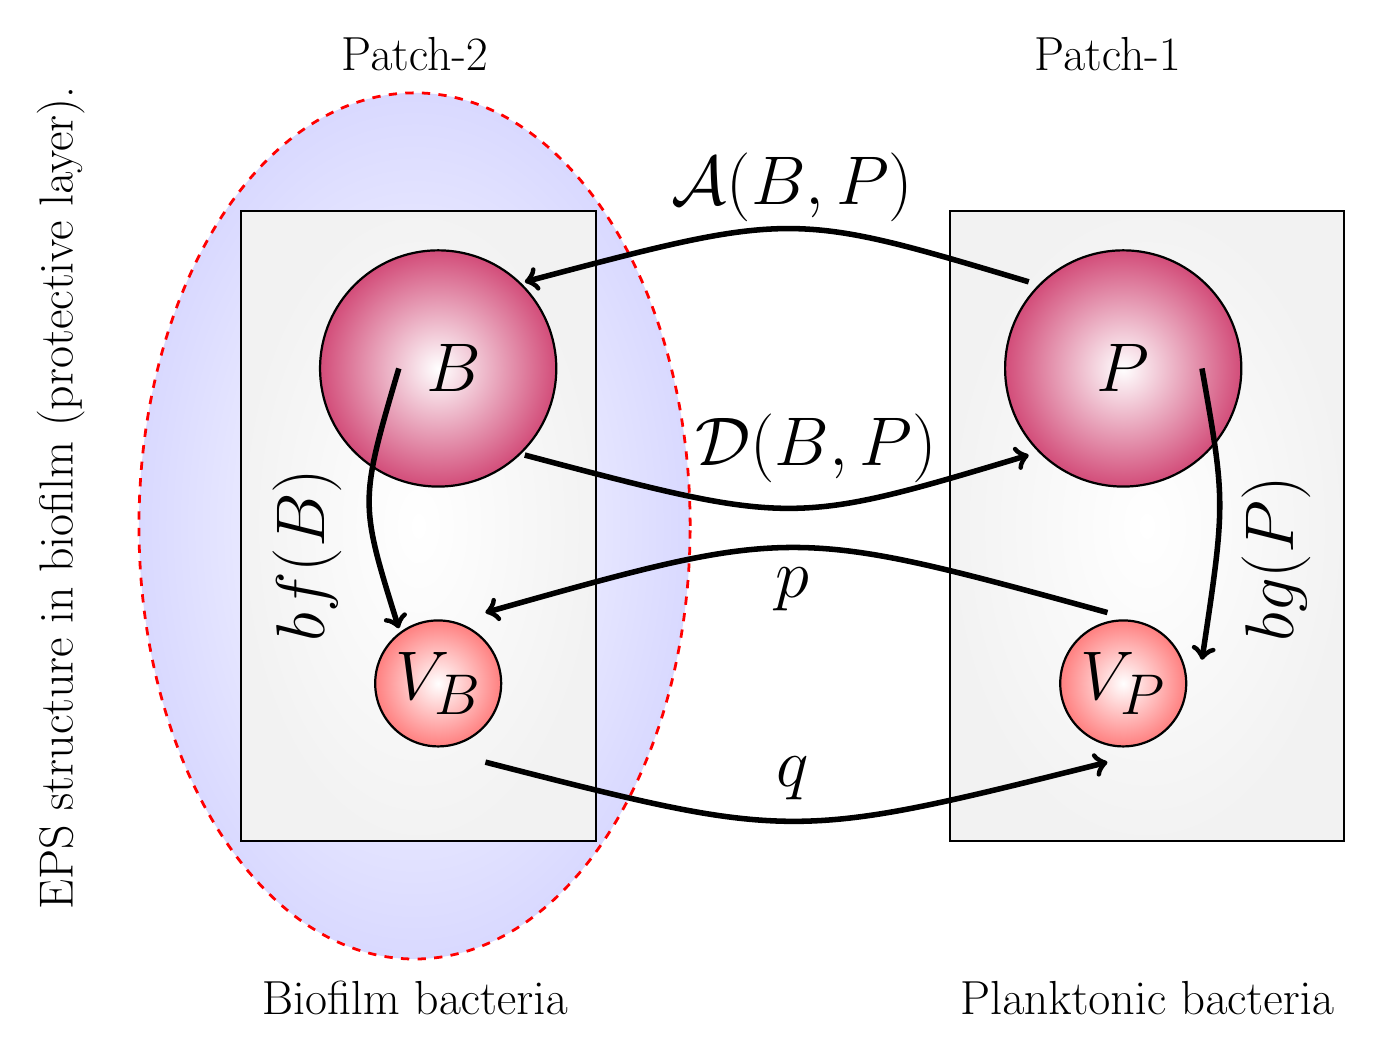
\begin{tikzpicture}[thick]
\draw [red, dashed,line width=1pt, shade, 
            outer color= blue!15!white, inner color=white, 
            align=center](-0.8,2) ellipse (3.5cm and 5.5cm);
\draw  [shade, outer color= black!5!white, inner color=white, 
            align=center](-3,-2) -- (1.5,-2) -- (1.5,6)-- (-3,6)--cycle;
\draw [shade, outer color= purple!70!white, inner color=white, 
            align=center](-0.5,4) circle  (1.5cm);
\draw [shade, outer color= red!50!white, inner color=white, 
            align=center](-0.5,0) circle  (0.8cm);
\draw [shade, outer color= black!5!white, inner color=white, 
            align=center](6,-2) -- (11,-2) -- (11,6)-- (6,6)--cycle;
\draw [shade, outer color= purple!70!white, inner color=white, 
            align=center](8.2,4) circle  (1.5cm);
\draw [shade, outer color= red!50!white, inner color=white, 
            align=center](8.2,0) circle  (0.8cm);
\node (a) at (-0.3,4) {\Huge $ B$};
\node (b) at (-0.5,0) {\Huge $ V_{B}$};
\node (c) at (8.2,4) {\Huge $ P $};
\node (d) at (8.2,0) {\Huge $V_P$};
\draw [->, line width =2pt]  (7, 5.1).. controls (4,6) .. (0.6,5.1);
\node (e) at (4,6.3) {\Huge ${\LARGE {\mathcal{A}(B,P)}}$};
\draw [->, line width = 2pt]  (0.6,2.9).. controls (4,2) ..(7, 2.9) ;
\node (f) at (4.3,2.99) {\Huge $\mathcal{D}(B,P)$};
\draw [->, line width =2pt]  (8, 0.9).. controls (4,2) .. (0.1,0.9);
\draw [->, line width =2 pt]  (0.1,-1.0).. controls (4,-2) .. (8, -1.0);
\draw [->, line width = 2pt]  (-1, 4).. controls (-1.5,2.3) .. (-1,0.7);
\draw [->, line width = 2pt]  (9.2, 4).. controls (9.5,2.3) .. (9.2,0.3);
\node (g) at (4,1.2) {\Huge $p$};
\node (h) at (4,-1.2) {\Huge $q$};
\node (i) at (-0.8,-4) {\LARGE Biofilm bacteria};
\node (i) at (-0.8,8) {\LARGE Patch-2};
\node (j) at (8.5, -4) {\LARGE Planktonic bacteria};
\node (i) at (8,8) {\LARGE Patch-1};
\node[label={[label distance=0.5cm,text depth=-1ex,rotate=90]right:\Huge $bf(B)$}] at (-2.4,-0.1) {};
\node[label={[label distance=0.5cm,text depth=-1ex,rotate=90]right:\Huge $ bg(P)$}] at (9.9,-0.1) {};
\node[label={[label distance=0.5cm,text depth=-1ex,rotate=90]right: {\LARGE EPS structure in biofilm (protective layer).}}] at (-5.5,-3.5) {};
\end{tikzpicture}
}
\caption[Diagram of the model.]{Diagram of the model. In patch-$1$ there is no group defence mechanism but prey (bacteria) can take refuge in patch-$2,$ where they can have group defence mechanism and can protect themselves against predator (phage).}\label{fig:patches}
\end{figure}\\

%In next section analysis of recently employed therapeutic strategies is carried out and is shown that although these therapeutic strategies can maximize the killing of bacteria in biofilm but can  not results in complete eradication of biofilm. We also suggest a therapeutic strategy which can result in complete eradication of biofilm and if there is no inherited resistance complete elimination of bacteria is possible. 

\section{Therapeutic strategies}
Recent experimental work has addressed approaches for minimizing or eradicating bacterial biofilms \citep{chaudhry_synergy_2017}.  In particular, Chaudhry {\it et al.} compared two therapeutic strategies: applying antibiotics and then phages, or applying the same two agents in the reverse order.  Treatment with phages first followed by antibiotics resulted in maximum killing of biofilm bacteria. Here we predict that although these strategies can indeed reduce the biofilm, neither strategy can eradicate the biofilm completely.

\subsection{Using antibiotics first and then phages}

Given that planktonic bacteria are many-fold more sensitive to antibiotics than biofilm bacteria, we assume that an appropriate antibiotic is administered such that planktonic bacteria can be effectively eliminated before phage therapy. We also assume that $\mathcal{A}(B,P)=\mathcal{D}(B, P).$ After the application of antibiotic we will arrive at the following system 
\begin{eqnarray}\label{modelb1}
\frac{dB}{dt} &=& r\left(1-\frac{B}{K_{B}}\right)B-f(B) V_{B} \nonumber\\
\frac{d V_{B}}{dt} &=& bf(B)V_{B}-cV_{B}.
\end{eqnarray}
This is a standard predator-prey system with group defense, as studied in  \citep{wolkowicz_bifurcation_1988, freedman_predator-prey_1986, zhu_bifurcation_2002,broer_predator-prey_2006}. In particular,   $f(B)$ must satisfy $f(0)=0, \, f(B)>0 \,\, \text{for all}\,\, B>0$, and if there exists a constant $M>0,$ such that 
$f^{'}(B)>0\,\, \text{if}\,\, B<M\, \, \text{and} \,\,f^{'}(B)<0 \,\, \text{if}\,\, B>M$, then the system models group defence \citep{freedman_predator-prey_1986}.
The  function $f(B)=\frac{m\,B}{\alpha \, B^{2}+ \beta \, B+1},$
called the Holling Type-IV or the Monod-Haldane function, was introduced in \citep{andrews_mathematical_1968} and satisfies these properties. System (\ref{modelb1}) has been previously studied with the above functional response for $\beta >-2\sqrt{\alpha}$  \citep{zhu_bifurcation_2002, jiang_multistable_2017}, and with $f(B) = \alpha e^{ -\beta B}$ \citep{xiao_global_2001}.\\

In this study, we consider biofilm bacteria that cannot exceed their carrying capacity, such that $B \leq K_{B}$ at all times. Hence  we replace the property 
$f(B)>0 \,\, \text{for all} \,\,B>0$ by 
$f(B)>0 \,\, \text{for all} \,\,0<B\le K_{B}$ . 
%$f(B)>0 \,\, \text{for all} \,\,0<B<\kappa K_{B}, \,\, %\text{where} \,\, 1<\kappa<2.$
 To model this phenomenon, we propose a relatively simple functional response 
 $f(B)=\alpha\left(\kappa-\frac{B}{K_{B}}\right)B.$
\textcolor{black}{The rationale for this function is similar to the rationale underpinning logistic growth: we assume that as the biofilm population
 approaches carrying capacity, the ability of phage to
 penetrate the biofilm is reduced, linearly.} The resulting functional response has the same properties as that of $f(B)$ defined in \citep{zhu_bifurcation_2002,xiao_global_2001} for $0<B \leq K_{B}$. 
 Here $\alpha$ is proportional to the adsorption rate of phages to bacteria, $1<\kappa<2$ is the group defense parameter, and $K_{B}$ is the carrying capacity of the biofilm bacteria. A convenient feature of this model is that the group defense mechanism can be controlled through the parameter $\kappa$; $\kappa=1$ corresponds to a perfect group defense mechanism \textcolor{black}{(no phage adsorption when the biofilm is at carrying capacity)} and $\kappa=2$ corresponds to the absence of effective group defense \textcolor{black}{($f(B)$ increasing on $0<B\le K_B$ )}.\\  

System (\ref{modelb1}) has a maximum of four equilibria. Two boundary equilibria are: $E_{0}=(0,0),$ which represents the complete extinction of biofilm bacteria and phages; and $E_{K_{B}}=(K_{B},0),$ which represents the extinction of phages while the biofilm bacteria reaches carrying capacity. In addition, two positive equilibria are: $E_{\mu_{1}}=(\mu_{1}, \mathcal{F}(\mu_{1}))$ and $E_{\mu_{2}}=(\mu_{2}, \mathcal{F}(\mu_{2}))$ subject to some conditions of existence. Here 
$\mathcal{F}(B)=\frac{r\big(1-\frac{B}{K_{B}}\big)}{\alpha\big(\kappa-\frac{B}{K_{B}}\big)}$
and $\mu_{1}$ and $\mu_{2}$ are solutions to the equation $\hat{f}(B)=\hat{c},$
where $\hat{f}(B)=\left (\kappa-\frac{B}{K_{B}}\right)\,B$ and $\hat{c}= \frac{c}{b\, \alpha}$
and $\mu_{1}<\frac{\kappa \, K_{B}}{2}<\mu_{2} <K_{B}.$
The existence of the two positive equilibria $E_{\mu_{1}}$ and $E_{\mu_{2}}$ depend on the positioning of the prey isocline $V_{B}=\mathcal{F}(B)$ and predator isoclines $B=\mu_{1}$ and $B=\mu_{2}$. As we increase $\hat{c}$ in the interval $(0, \hat{c}_{M})$, $\mu_{1}$ and $\mu_{2}$ become closer to each other; when $\hat{c}=\hat{c}_{M}$ the two equilibria coincide and we get
$E_{\mu_{1}}=E_{\mu_{2}}=\left(\frac{\kappa \, K_{B}}{2}, \frac{r\left(1-\frac{\kappa}{2}\right)}{\alpha \left(\kappa-\frac{\kappa}{2}\right)}\right).$
Equilibria and their existence can be summarized in the following theorem.
\begin{theorem}
System (\ref{modelb1}) has four equilibria $E_{0},$ $E_{K_{B}},$ $E_{\mu_{1}}$ and $E_{\mu_{2}}$ if $\hat{c} \in (\hat{c}_{m}, \hat{c}_{M}),$ three equilibria $E_{0},$ $E_{K_{B}}$ and $E_{\mu_{1}}$ if $\hat{c} \in (0, \hat{c}_{m}),$ three  equilibria $E_{0},$ $E_{K_{B}}$ and $E_{\mu_{1}}=E_{\mu_{2}}=E_{\mu}=\left(\frac{\kappa \, K_{B}}{2}, \frac{r\left(1-\frac{\kappa}{2}\right)}{\alpha \left(\kappa-\frac{\kappa}{2}\right)}\right)$ if $\hat{c}=\hat{c}_{M},$ only two equilibria $E_{0}$ and $E_{K_{B}}$ if $\hat{c} > \hat{c}_{M},$
where $\hat{c}=\frac{c}{b\, \alpha},$ $\hat{c}_{M}=\frac{\kappa^{2}}{4}K_{B}$ and $\hat{c}_{m}= (\kappa-1)K_{B}.$
\end{theorem}

\subsubsection{Stability analysis}
It can be easily shown that $E_{0}=(0,0)$ has eigenvalues
$\lambda_{1}=r>0, \,\, \lambda_{2}=-c<0$
showing that $E_{0}=(0,0)$ is a saddle point. The equilibria $E_{K_{B}}=(K_{B},0)$ has
$\lambda_{1}=-r, \,\, \lambda_{2}=b\alpha(\hat{c}_{m}-\hat{c}),$ as eigenvalues, showing that $E_{K_{B}}$ is an attractive node, if $\hat{c}>\hat{c}_{m},$ and is a saddle point if $\hat{c}< \hat{c}_{m}.$ To study the stability of the other two equilibria, if they exist, we write the model (\ref{modelb1}) as
\begin{eqnarray}\label{modeb11}
\frac{dB}{dt} &=& f(B)\left(\mathcal{F}(B)- V_{B}\right)\nonumber\\
\frac{d V_{B}}{dt} &=& bf(B)V_{B}-cV_{B}.
\end{eqnarray}
The eigenvalues for $E_{\mu_{1}}$ are $\lambda_{1,2}=\frac{\xi_{1}\pm\sqrt{\xi_{1}^{2}-4\Delta_{1}}}{2},$ where
$\xi_{1}=f(\mu_{1})\mathcal{F}^{'}(\mu_{1})$
is the trace of Jacobian matrix of (\ref{modeb11}) at $E_{\mu_{1}}.$ Since $\mathcal{F}^{'}(B)<0,$ hence $\xi_{1}<0$ and 
$\Delta_{1} = b \, \alpha^{2}\, \mu_{1} \left(\kappa-\frac{\mu_{1}}{K_{B}}\right)\left(\kappa - \frac{2\, \mu_{1}}{K_{B}}\right)$
is the determinant of the Jacobian matrix at $E_{\mu_{1}}.$ As $\mu_{1}<\frac{\kappa K_{B}}{2},$ hence $\Delta_{1}>0.$ This demonstrates that $E_{\mu_{1}}$ is an attracting point. Similarly, the eigenvalues corresponding to $E_{\mu_{2}}$ are $\lambda_{1,2}=\frac{\xi_{2} \pm \sqrt{\xi_{2}^{2}-4\Delta_{2}}}{2},$
where $\xi_{2}=f(\mu_{2})\mathcal{F}^{'}(\mu_{2})<0$
is the trace of Jacobian matrix at $E_{\mu_{2}}$ and $\Delta_{2}= b \, \alpha^{2}\, \mu_{2} \left(\kappa-\frac{\mu_{2}}{K_{B}}\right)\left(\kappa - \frac{2\, \mu_{2}}{K_{B}}\right)<0$
is the determinant of the Jacobian matrix at $E_{\mu_{2}}.$ We conclude that $E_{\mu_{2}}$ is a saddle point.  Since only one equilibrium corresponds to the extinction of biofilm bacteria, and it is a saddle point for all feasible  parameter values, we conclude that complete eradication of the biofilm is not possible using this therapeutic strategy. {\color{black} This conclusion is consistent with the view, as discussed in an extensive review \citep{abedon_ecology_2015II}, that phage action is not sufficient for complete eradication of biofilms.}

\subsection{Using phages first and then antibiotics}
In order to understand phage therapy, we return to model (\ref{modelb}), approximating the complicated processes of attachment and detachment by simpler functions to gain tractability. Specifically, we assume biofilm bacteria detach at constant per capita rate $n$; \textcolor{black}{this
assumption has a long history in the literature, extending back to Freter's influential research on bacterial colonization of the intestinal tract \citep{freter_survival_1983,jones_freter_2003}.}  We further assume that planktonic bacteria attach at constant per capita rate $m$. \textcolor{black}{In Freter's original biofilm model, attachment is also proportional to the number of planktonic bacteria, but is further restricted by the number of available ``wall attachment sites'' \citep{freter_survival_1983}.  In our model, we restrict biofilm \emph{growth} by the number of attachment sites, $K_B$, but take a linear
attachment rate.} Since $B$ and $P$ are densities (cells per unit volume), the net transfer of cells between compartments must be scaled, yielding  $\mathcal{A}(B,P) = \left(\frac{vol_ {_{P}}}{vol_{_{B}}}\right)\, m\, P$ and $\mathcal{D}(B,P)=\left(\frac{vol_ {_{B}}}{vol_{_{P}}}\right)\, n\,B$, where $vol_B$  and $vol_P$ are the volumes of the biofilm and planktonic compartments respectively.  After the substitution of these function into system (\ref{modelb}), it can be shown by direct calculation that the resulting system has three equilibrium solutions: the trivial equilibrium, an equilibrium with both classes of bacteria only, and the all-existing equilibrium (exact expressions omitted for brevity).
%\begin{equation}\label{Eqn50}  
%\begin{array}{ll}  
%%{\rm E_0}: (B,P,V_B,V_P) = (0,0,0,0), \\
%{\rm E_1}: (B,P,V_B,V_P) = (B^{*}, P^{*}, 0, 0 ),\\
%{\rm E_2}: (B,P,V_B,V_P) = \big( %B^{**},P^{**},V_B^{**},V_P^{**} \big).
%\end{array} 
%\end{equation} 
%\subsubsection{Stability analysis}
Out of these equilibria the only equilibrium which corresponds to the complete eradication of biofilm bacteria is $\rm E_0.$ It can be shown by a direct calculation that this equilibrium $\rm E_0$ is a saddle point for all feasible parameter values. This demonstrates that phage therapy will not eradicate the biofilm.  Since the biofilm bacteria are resistant to antibiotics, we can conclude that even phage therapy followed by antibiotics will not remove the biofilm.

\subsection{A novel therapeutic strategy: blocking attachment}\label{3}
The model developed here allows us to address the following question: is there a therapeutic strategy, {\it in principle}, that could eradicate the biofilm?  Since attachment of planktonic bacteria is critical to biofilm maintenance, we investigated the model assuming this attachment is negligible, and phage therapy is also applied.
In this case it can be shown by direct calculations that system (\ref{modelb}), with the substitutions $\mathcal{A}(B,P)=0$ and $\mathcal{D}(B,P)=\left(\frac{vol_ {_{B}}}{vol_{_{P}}}\right)\, n\,B$, has five equilibrium solutions: 
\begin{equation}\label{Eqn52}  
\begin{array}{ll}  
{\rm E_0}: & (B,P,V_B,V_P) = (0,0,0,0) \\[0.5ex]  
{\rm E_1}: & (B,P,V_B,V_P) = (0,K_{P},0,0) \\[0.5ex]  
{\rm E_2}: & (B,P,V_B,V_P) = \big(0, 
\frac {c \left( c+p+q \right) }{\alpha\,b \left( c+q \right) }, 
\textstyle\frac{M\,p\, r} {b\alpha^2 (c+q)^2 K_P} 
 (\frac{vol_P}{vol_B}), \frac{M\,r}{b \alpha^2 K_P} 
\big),  \\[0.5ex]  
{\rm E_3}: & (B,P,V_B,V_P) = (B^*,P^*, 0, 0 ),  \\[0.5ex]  
{\rm E_4}: & (B,P,V_B,V_P) = \big( B^{**},P^{**},V_B^{**},V_P^{**} \big), 
\end{array} 
\end{equation} 
where 
\begin{equation}\label{Eqn3}  
M= b q \alpha K_P - c (c+p+q - b \alpha K_P) .
\end{equation}
Three of these equilibria, ${\rm E_{0}}, {\rm E_{1}}$ and ${\rm E_{2}}$, represent complete eradication of the biofilm. The equilibria ${\rm E_0}$ and ${\rm E_1}$ exist for any positive parameter values, while ${\rm E_2}$ exists only for $M \ge 0,$ i.e. $\alpha \ge \frac{c(c+p+q)}{b K_{P} (c+q)}.$ The equilibrium ${\rm E_{0}}$ is a saddle point for all feasible values of parameters. The equilibrium ${\rm E_{1}}$ is asymptotically stable if $n>r$ and $ \alpha <\frac{c\left(c+p+q\right)}{b\,K_{P}(c+q)}.$   This implies that if the detachment rate is greater than the birth rate of bacteria in the biofilm and adsorption rate is less than $\frac{c\left(c+p+q\right)}{b\,K_{P}(c+q)}$, then elimination of biofilm bacteria is possible; in particular, planktonic bacteria will reach their carrying capacity and there will be no biofilm or planktonic viruses.   Using the Hurwitz criterion, it can be shown that the equilibrium ${\rm E_2}$ is stable if $ M > 0 ,$  i.e. 
$\alpha >\frac{c\left(c+p+q\right)}{b\, K_{P}(c+q)}$ (which guarantees its existence), and   $n > \text{max}(0, \bar{N_{1}}),$ where $$\bar{N_{1}}=r 
- \frac{r \kappa p (\frac{vol_P}{vol_B})\, M}{ b \alpha (c+q)^2 K_P}.$$ If $\bar{N_{1}}$ is negative, the conditions for elimination of the biofilm become $n>0$ and $\alpha >\frac{c\left(c+p+q\right)}{b\, K_{P}(c+q)}$.  Thus, the model predicts that biofilm eradication is possible if the attachment of planktonic bacteria to the biofilm, $\mathcal{A}(B,P)$ can be blocked. \textcolor{black}{Although an analysis of 
realistic numerical parameter values is outside the scope of this contribution, we note that the rate at which the biofilm
could be eliminated depends on the difference between the logistic growth rate, $r$, and the loss rate of biofilm $(f(B)V_B - \mathcal{D}(B,P))/B$.}

\section{Summary and Conclusions}

Biofilm formation starts with the attachment of planktonic (free-living) bacteria to a surface. As these bacteria become sessile and start producing the extracellular matrix (EPS) which defines the biofilm, other bacteria from the planktonic state continue to attach. In this way the bacteria develop a colony that can minimize the infiltration of antibacterial agents. In particular, antibiotics are often ineffective against biofilms, both due to the extracellular structure and the presence of persister cells, which are metabolically inactive. Phages (viruses that infect bacteria) offer the most promising alternative strategy for removing biofilms. Some phages such as T4 can easily infiltrate the EPS structure and can also infect and kill persister cells \citep{harper_bacteriophages_2014}.

%In \citep{tait_efficacy_2002} the author claimed the complete elimination of a single species \textit{Enterobacter cloacae} biofilm using phages. It was also claimed in the same study that phages are less effective against multi-species biofilm.
A range of experimental studies have shown that phages, antibiotics or other agents alone are not enough to eradicate a biofilm completely, hence a combination of these agents is typically recommended \citep{chaudhry_synergy_2017, ryan_synergistic_2012}.
In this study we derive a mathematical model which predicts that a combination of antibiotics and phage therapy cannot eradicate a biofilm, whether applied as antibiotics followed by phage, or in the reverse order, as studied in \citep{chaudhry_synergy_2017}. 

In subsection \ref{3}, we investigate a novel, hypothetical therapeutic strategy.  In particular, we demonstrate that if further attachment of planktonic bacteria to the biofilm can be blocked (even if the biofilm is already mature), complete elimination of the biofilm is possible using phages.  After eliminating the biofilm, antibiotics can be used to eliminate any remaining planktonic bacteria.  This result suggests that blocking attachment, perhaps by blocking EPS production, is a promising avenue for biofilm eradication.  Interestingly, the genetic pathways associated with quorum sensing may in fact be the targets of several natural biofilm inhibitors \citep{lee_low_2011}.%jakobsen_ajoene_2012}.  Since quorum sensing is a precursor for aggregation in many species, this suggests that processes analogous to attachment in our model may be blocked by these historical antimicrobial agents. 

Mathematically, the model we derive is a two-patch predator-prey system with group defense by the prey in one patch.  Our analysis was made tractable by proposing a simple, novel functional response describing group defense.  While this function is invalid (become negative) for biofilm densities that exceed an upper bound, in reality physical constraints limit the density of cells in biofilms, and this limitation did not impede analysis.  We expect that this functional form may have further uses in the study of group defense mechanisms, particularly when other aspects of the model become more complex.

%Presently employed techniques can be used to overcome phenotypic resistance but inherited resistance, although being secondary, is much bigger challenge. There are various factors responsible for the inherited or genotypic resistance and further investigation of these factors is required inorder to develop a best strategies to deal with inherited resistance of bacteria.


\addcontentsline{toc}{chapter}{Bibliography}
\bibliographystyle{abbrv}
\bibliography{refrence}
